\documentclass[10pt,aspectratio=169]{beamer}
\usetheme{metropolis}
\usepackage{booktabs}
\usepackage{amssymb}
\usepackage{siunitx}
\usepackage{graphicx}
\usepackage{xcolor}
\usepackage{tikz}
\usetikzlibrary{shapes.geometric, arrows.meta, positioning, fit, backgrounds, matrix, decorations.pathreplacing}
\definecolor{good}{HTML}{2E7D32}
\definecolor{bad}{HTML}{C62828}
\definecolor{llmblue}{HTML}{1565C0}
\newcommand{\gd}[1]{\textcolor{good}{#1}}
\newcommand{\bd}[1]{\textcolor{bad}{#1}}
\metroset{block=fill}

\tikzset{
  ai/.style={rectangle, rounded corners, draw=llmblue, line width=0.9pt, fill=llmblue!8, align=center, font=\small, inner sep=6pt},
  frozen/.style={rectangle, rounded corners, draw=good, line width=1.0pt, fill=good!10, align=center, font=\small, inner sep=6pt},
  data/.style={rectangle, draw=gray!70, fill=gray!8, align=center, font=\footnotesize\ttfamily, inner sep=5pt},
  gate/.style={diamond, aspect=2, draw=bad, line width=1.0pt, fill=bad!8, align=center, font=\footnotesize, inner sep=1pt},
  arr/.style={-{Stealth[length=2.5mm]}, line width=0.9pt, gray!70},
}

\title{Centri --- Making the Numbers Trustworthy}
\subtitle{A plain-language walkthrough of the recent overhaul}
\author{NCU HwangLab \\ Damar \& Claude Opus 4.8}
\date{Companion to the technical report --- Jun 2026}

\begin{document}

\maketitle

\begin{frame}{The story in one slide}
\begin{itemize}
  \item \textbf{What Centri does:} you film an object spinning on a turntable; the app measures its rotation --- angular speed $\omega$, period, velocity --- straight from the video.
  \item \textbf{The problem we found:} feeding the \emph{exact same video} twice gave \emph{different answers}, sometimes badly different, sometimes a broken results file.
  \item \textbf{Why:} the AI was re-inventing the physics calculation on every single run.
  \item \textbf{The fix:} let the AI do what it's good at (\emph{looking} at the video), and hand the \emph{math} to fixed, vetted code that can never change.
  \item \textbf{The outcome:} same video $\to$ \gd{identical answer, every time}, and within \gd{0.2--0.4\%} of a phone's gyroscope.
\end{itemize}
\end{frame}

\section{The problem}

\begin{frame}{Same video in, different answer out}
We dug up 30 past runs. The results were all over the place:
\centering\small
\begin{tabular}{lcccc}
\toprule
Video & runs & rotation period (s) & spread & valid results file? \\
\midrule
IMG\_3071 & 15 & \bd{0.79 -- 1.00} & \bd{26\%} & often broken \\
IMG\_3072 & 5  & 1.486 -- 1.487 & 0\% & often broken \\
IMG\_3075 & 5  & 1.102 & 0\% & often broken \\
\bottomrule
\end{tabular}
\par\vspace{0.6em}
\begin{itemize}\footnotesize
  \item Across the 30 runs the results file came in \bd{28 different layouts} --- and \bd{17 were technically broken} (contained \texttt{NaN}, i.e. ``not a number'', which isn't valid data).
  \item For a teaching tool, this is fatal: a student could run the same clip twice and be told two different physics answers.
\end{itemize}
\end{frame}

\begin{frame}{Why it happened --- an analogy}
\begin{block}{The mistake}
We had asked the AI to \emph{both} watch the video \emph{and} write the physics maths fresh, every run. It's like hiring a brilliant assistant and asking them to re-derive the formula for kinetic energy from scratch on every homework problem --- they'll get it slightly different (or wrong) each time.
\end{block}
\begin{block}{The insight}
\emph{Looking} at a video is genuinely a judgment task --- which object? where's the centre of rotation? how big is it? That \emph{should} be the AI's job.

\emph{Computing} $\omega$ and period from a known set of points is just arithmetic. There is one right answer, and it should never vary.
\end{block}
\end{frame}

\section{The fix}

\begin{frame}{One clean seam: the AI looks, fixed code computes}
\centering
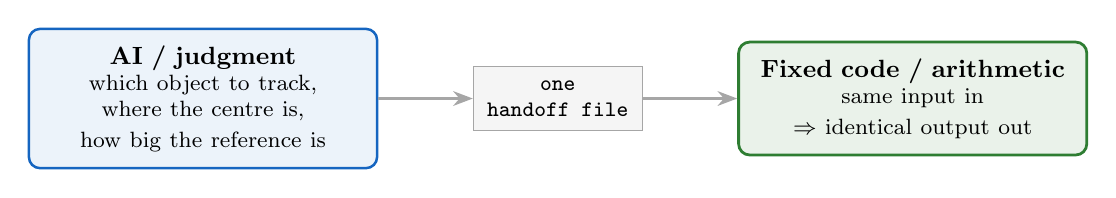
\begin{tikzpicture}[node distance=8mm]
\node[ai, text width=4.0cm] (a) {\textbf{AI / judgment}\\ \footnotesize which object to track,\\ where the centre is,\\ how big the reference is};
\node[data, right=12mm of a] (c) {one\\handoff file};
\node[frozen, right=12mm of c, text width=4.0cm] (f) {\textbf{Fixed code / arithmetic}\\ \footnotesize same input in\\ $\Rightarrow$ identical output out};
\draw[arr] (a)--(c); \draw[arr] (c)--(f);
\end{tikzpicture}
\par\vspace{0.8em}
\begin{itemize}\footnotesize
  \item The AI's job now \emph{ends} when it writes that one handoff file describing what it saw.
  \item Everything downstream --- cleaning the data, fitting the circle, computing speed, finding the period --- runs through \gd{frozen code that the AI is forbidden to touch or rewrite}.
  \item This code is version-controlled and reviewed once, then copied unchanged into every job.
\end{itemize}
\end{frame}

\begin{frame}{The whole journey, end to end}
\centering
\resizebox{\textwidth}{!}{%
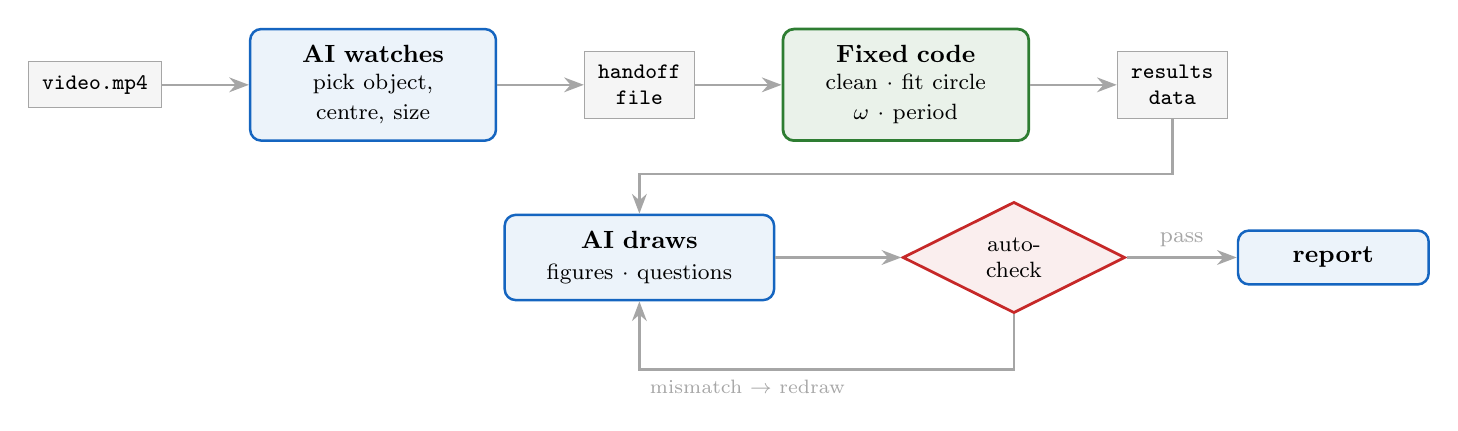
\begin{tikzpicture}[node distance=7mm and 11mm]
\node[data] (vid) {video.mp4};
\node[ai, right=of vid, text width=2.7cm] (perc) {\textbf{AI watches}\\\footnotesize pick object,\\ centre, size};
\node[data, right=of perc] (contract) {handoff\\file};
\node[frozen, right=of contract, text width=2.7cm] (run) {\textbf{Fixed code}\\\footnotesize clean $\cdot$ fit circle\\ $\omega$ $\cdot$ period};
\node[data, right=of run] (stats) {results\\data};
\draw[arr] (vid)--(perc); \draw[arr] (perc)--(contract); \draw[arr] (contract)--(run); \draw[arr] (run)--(stats);

\node[ai, below=12mm of contract, text width=3.0cm] (subs) {\textbf{AI draws}\\\footnotesize figures $\cdot$ questions};
\node[gate, right=16mm of subs, text width=1.6cm] (gate) {auto-\\check};
\node[ai, right=14mm of gate, text width=2.0cm] (rep) {\textbf{report}};
\draw[arr] (stats.south) -- ++(0,-7mm) -| (subs.north);
\draw[arr] (subs)--(gate);
\draw[arr] (gate)-- node[above,font=\footnotesize]{pass} (rep);
\draw[arr] (gate.south) -- ++(0,-7mm) -| node[below right,font=\scriptsize]{mismatch $\to$ redraw} (subs.south);
\end{tikzpicture}}
\par\vspace{0.6em}
\footnotesize \textcolor{llmblue}{Blue = AI / judgment (can vary)} \qquad \gd{Green = fixed code (always identical)} \qquad \texttt{grey = data}.
\par The AI only ever \emph{looks} and \emph{draws}; every number comes from the green box.
\end{frame}

\begin{frame}{What ``frozen code'' buys us --- three guarantees}
\begin{block}{1. The circle fit can't wander}
The step that fits a circle to the tracked points now uses a fixed random seed --- so it produces the \emph{exact same fit} every time, not a slightly different one each run.
\end{block}
\begin{block}{2. One source of truth for angular speed}
$\omega$ is computed \emph{once} and reused everywhere (summary, period, phases). The old code computed it two different ways that disagreed.
\end{block}
\begin{block}{3. The results file has a locked format}
Always the same fields, and a stray ``not a number'' now \bd{stops the run} instead of silently shipping a broken file.
\end{block}
\end{frame}

\section{Results}

\begin{frame}{Now: same video $\to$ identical answer, and it's accurate}
We re-ran each video three times. Compared against a phone gyroscope (ground truth the AI never sees):
\centering\small
\begin{tabular}{lcccc}
\toprule
Video & period (s) & $\omega$ (rad/s) & vs.\ gyroscope & repeatable? \\
\midrule
IMG\_3071 & \gd{0.839} & \gd{7.372} & \gd{0.2\%} & \gd{identical $\times$3} \\
IMG\_3072 & \gd{1.438} & \gd{4.827} & \gd{0.4\%} & \gd{identical $\times$3} \\
IMG\_3075 & 1.10 -- 1.15 & 5.79 -- 5.89 & \gd{0.3\%} & 2 of 3 identical \\
\bottomrule
\end{tabular}
\par\vspace{0.7em}
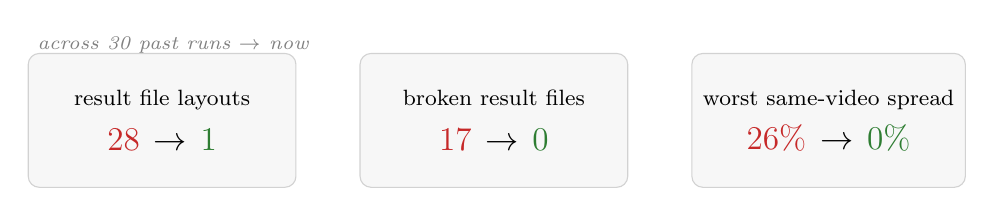
\begin{tikzpicture}[
  card/.style={rectangle, rounded corners, draw=gray!35, fill=gray!6, minimum width=3.4cm, minimum height=1.7cm, align=center, inner sep=4pt},
  node distance=8mm]
\node[card] (c1) {\footnotesize result file layouts\\[4pt] {\large \bd{28}}\ \,{\large $\to$}\ \,{\large \gd{1}}};
\node[card, right=of c1] (c2) {\footnotesize broken result files\\[4pt] {\large \bd{17}}\ \,{\large $\to$}\ \,{\large \gd{0}}};
\node[card, right=of c2] (c3) {\footnotesize worst same-video spread\\[4pt] {\large \bd{26\%}}\ \,{\large $\to$}\ \,{\large \gd{0\%}}};
\node[above=1mm of c1.north west, anchor=west, font=\scriptsize\itshape, text=gray] {across 30 past runs $\to$ now};
\end{tikzpicture}
\par\vspace{0.5em}
\footnotesize The small residual wobble on IMG\_3075 is the \emph{camera tracking} drawing a slightly different path that run --- \emph{not} the maths. The AI-looks / fixed-code-computes split now lets us tell the two apart.
\end{frame}

\begin{frame}{Why jobs got faster: the physics code isn't written each run}
\centering
\resizebox{0.96\textwidth}{!}{%
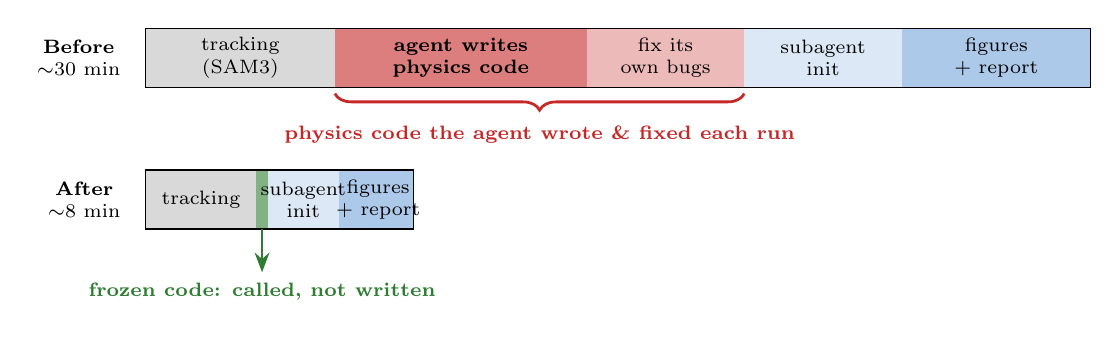
\begin{tikzpicture}[font=\scriptsize, every node/.style={align=center}]
\def\h{0.75}
% ---- BEFORE bar ----
\fill[gray!30]    (0,2.0)  rectangle (2.4,2.0+\h);
\fill[bad!60]     (2.4,2.0) rectangle (5.6,2.0+\h);
\fill[bad!32]     (5.6,2.0) rectangle (7.6,2.0+\h);
\fill[llmblue!15] (7.6,2.0) rectangle (9.6,2.0+\h);
\fill[llmblue!35] (9.6,2.0) rectangle (12.0,2.0+\h);
\draw (0,2.0) rectangle (12.0,2.0+\h);
\node[anchor=east] at (-0.2,2.0+\h/2) {\textbf{Before}\\ $\sim$30 min};
\node at (1.2,2.0+\h/2) {tracking\\ (SAM3)};
\node at (4.0,2.0+\h/2) {\textbf{agent writes}\\ \textbf{physics code}};
\node at (6.6,2.0+\h/2) {fix its\\ own bugs};
\node at (8.6,2.0+\h/2) {subagent\\ init};
\node at (10.8,2.0+\h/2) {figures\\ + report};
% brace under the removed band
\draw[decorate, decoration={brace, amplitude=6pt, mirror}, bad, line width=1pt]
  (2.4,1.92) -- (7.6,1.92);
\node[bad, font=\scriptsize\bfseries] at (5.0,1.4) {physics code the agent wrote \& fixed each run};
% ---- AFTER bar ----
\fill[gray!30]    (0,0.2) rectangle (1.4,0.2+\h);
\fill[good!60]    (1.4,0.2) rectangle (1.55,0.2+\h);
\fill[llmblue!15] (1.55,0.2) rectangle (2.45,0.2+\h);
\fill[llmblue!35] (2.45,0.2) rectangle (3.4,0.2+\h);
\draw (0,0.2) rectangle (3.4,0.2+\h);
\node[anchor=east] at (-0.2,0.2+\h/2) {\textbf{After}\\ $\sim$8 min};
\node at (0.7,0.2+\h/2) {tracking};
\node at (2.0,0.2+\h/2) {subagent\\ init};
\node at (2.95,0.2+\h/2) {figures\\ + report};
\draw[arr, good, line width=0.9pt] (1.475,0.2) -- ++(0,-0.55)
  node[below, good, font=\scriptsize\bfseries] {frozen code: called, not written};
\end{tikzpicture}}
\par\vspace{0.4em}
\footnotesize
Before, the agent \textbf{wrote the physics calculation from scratch each run} --- turning SAM3 position data into $\omega$, period, etc.\ --- and sometimes had to fix its own bugs. Preseeding the \gd{frozen library removes that step}: the math is \emph{called}, not generated. Tracking, subagents and the report are otherwise unchanged. \emph{(schematic --- segment widths illustrative, not measured.)}
\end{frame}

\section{What we caught along the way}

\begin{frame}{Determinism made bugs reproducible --- so we could finally fix them}
\begin{block}{Bug 1: the circle fit latched onto a giant phantom circle}
On one video the fit chose a huge, nearly-straight arc (radius 3.1\,m for a desktop turntable!), which then threw away half the real data. \gd{Fix:} measure the radius from the trusted centre instead, and reject physically implausible fits. $\omega$ went from \bd{0.0} (broken) to \gd{7.372} (matches gyro).
\end{block}
\begin{block}{Bug 2: hand-converting between full-frame and cropped coordinates}
The AI was manually shifting points between the full video frame and a cropped region --- and did it inconsistently between runs, swinging one metric by \bd{81\%}. \gd{Fix:} that conversion now lives in the frozen code and is done for every point the same way. \emph{Whole class of bug is now structurally impossible.}
\end{block}
\end{frame}

\begin{frame}{The figures had to match the data too}
\footnotesize The chart-drawing step was reading points from one file and the centre from another --- so the fitted circle floated off the actual trajectory. We added an automatic check that compares every plotted figure against the real numbers and \bd{rejects} mismatches before the report is built.
\begin{columns}[T]
\begin{column}{0.5\textwidth}\centering
\bd{Before --- circle off the points}\\\includegraphics[height=0.6\textheight]{/tmp/v2_trajectory.png}
\end{column}
\begin{column}{0.5\textwidth}\centering
\gd{After --- circle on the points}\\\includegraphics[height=0.6\textheight]{/tmp/v3_trajectory.png}
\end{column}
\end{columns}
\end{frame}

\begin{frame}{How a bad figure gets stopped automatically}
\centering
\resizebox{0.92\textwidth}{!}{%
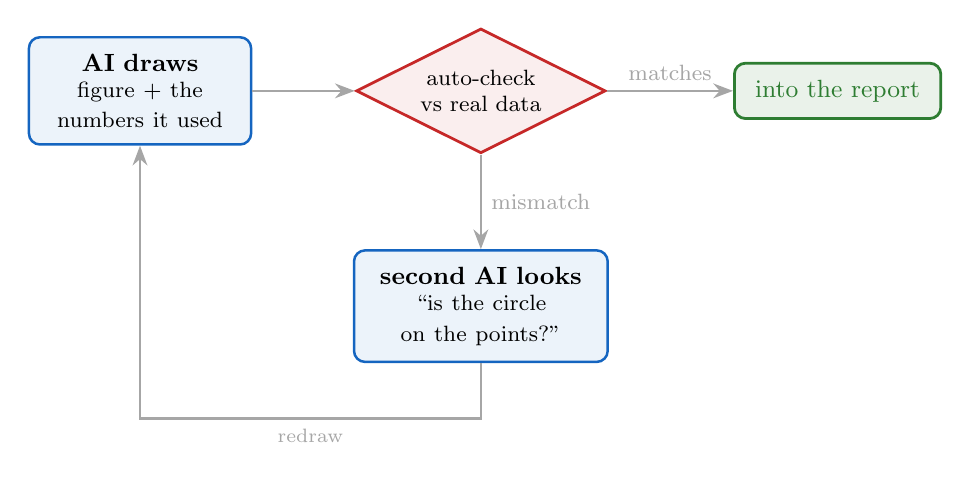
\begin{tikzpicture}[node distance=8mm and 13mm]
\node[ai, text width=2.4cm] (b) {\textbf{AI draws}\\\footnotesize figure + the\\ numbers it used};
\node[gate, right=of b, text width=1.9cm] (det) {auto-check\\vs real data};
\node[frozen, right=16mm of det, text width=2.2cm] (ok) {\gd{into the report}};
\node[ai, below=12mm of det, text width=2.8cm] (vqa) {\textbf{second AI looks}\\\footnotesize ``is the circle\\ on the points?''};
\draw[arr](b)--(det);
\draw[arr](det)--node[above,font=\footnotesize]{matches}(ok);
\draw[arr](det.south)--node[right,font=\footnotesize]{mismatch}(vqa);
\draw[arr](vqa.south) -- ++(0,-7mm) -| node[below,font=\scriptsize,pos=0.25]{redraw} (b.south);
\end{tikzpicture}}
\par\vspace{0.5em}
\footnotesize
The fast \textbf{auto-check} runs on \emph{every} job and compares the figure's claimed bounds against the real data --- instant, deterministic. Only if it fails do we spend a \textbf{second AI} to look at the picture and feed advice into the redraw. Correctness is \emph{enforced}, not hoped for.
\end{frame}

\section{Robustness}

\begin{frame}{Handling motion blur honestly}
When the object spins fast it blurs, and the tracker drops a few frames --- leaving gaps in the angular-speed curve.
\begin{center}
\includegraphics[width=0.9\textwidth]{/tmp/omega_beforeafter.png}
\end{center}
\vspace{-0.3em}
\footnotesize
We bridge only \emph{short} interior gaps ($\le$\SI{0.2}{s}), and only between two real detections, by following the circular path the object is on. Long gaps are left honest. The repair is deterministic and flagged in the data, so coverage always reflects what was actually seen.
\par\vspace{0.3em}
\textbf{Next step:} fill \emph{larger} gaps with interpolation / Kalman filtering --- \gd{without changing any real measurement} (the velocity peaks must stay identical).
\end{frame}

\begin{frame}{Does it generalise? A bicycle wheel}
\begin{columns}[T]
\begin{column}{0.58\textwidth}\centering
\includegraphics[width=0.49\linewidth]{/home/damar/centri/screenshot/bike-1.png}\hfill
\includegraphics[width=0.49\linewidth]{/home/damar/centri/screenshot/bike-2.png}
\par\footnotesize A marker on a spinning bicycle wheel --- tracked point, fitted circle, radius vector.
\end{column}
\begin{column}{0.42\textwidth}\footnotesize
\begin{tabular}{ll}
\toprule
direction & \gd{clockwise, correctly signed} \\
$\omega$ & $-5.12$ rad/s \\
period & 1.18 s \\
coverage & 93.8\% \\
\bottomrule
\end{tabular}
\par\vspace{0.5em}
A completely different geometry, no turntable --- and the same frozen pipeline resolves direction, speed and period correctly.
\par\vspace{0.3em}
\footnotesize (Without a known size, only $\omega$/period are exact; linear speed is scale-shifted --- expected.)
\end{column}
\end{columns}
\end{frame}

\section{The app}

\begin{frame}{App side: more reliable and friendlier}
\begin{itemize}
  \item \textbf{Auto-detect actually works now:} the ``find the object for me'' button used to hit a dead server (just errored on the phone). Fixed, and now the AI \emph{names} the object and a precise detector \emph{draws a tight box} around it --- in one tap.
  \item \textbf{Plain language for classrooms:} internal jargon (model names, ``reference ruler'') reworded into student/teacher-friendly terms; the size reference is now just \emph{the spinning platform itself}.
  \item \textbf{Nicer feedback:} live upload progress bar, readable history (friendly titles, ``2 min ago'', \texttt{2m\,54s} timings) instead of raw IDs.
  \item \textbf{Safety net:} one job once got stuck in a runaway loop and wrote an \bd{11\,GB} log; there's now a guard that stops it in 1--2 minutes and compresses logs.
  \item \textbf{Speed:} a full job dropped from \bd{$\sim$30 min} to \gd{$\sim$8 min}.
\end{itemize}
\end{frame}

\begin{frame}{The app in the student's hands}
\begin{columns}[T]
\begin{column}{0.33\textwidth}\centering
\includegraphics[height=0.74\textheight]{/home/damar/centri/screenshot/1.png}\\
\scriptsize Home --- record or pick a video
\end{column}
\begin{column}{0.33\textwidth}\centering
\includegraphics[height=0.74\textheight]{/home/damar/centri/screenshot/2.png}\\
\scriptsize History --- friendly titles \& timings
\end{column}
\begin{column}{0.33\textwidth}\centering
\includegraphics[height=0.74\textheight]{/home/damar/centri/screenshot/3.png}\\
\scriptsize Live analysis --- staged progress
\end{column}
\end{columns}
\end{frame}

\section{Honesty \& next steps}

\begin{frame}{What's solid, and what isn't yet}
\begin{block}{Solid}
Same video gives an identical, correct answer; agreement with the phone gyroscope is \gd{0.2--0.4\%}; every coordinate conversion now lives in fixed code; figures are checked against the data automatically.
\end{block}
\begin{block}{Still open --- honestly}
\begin{itemize}\footnotesize
  \item The \emph{tracking} of the object is still a bit non-deterministic --- the remaining run-to-run wobble comes from there, not the maths.
  \item One metric (\texttt{stable\_omega}) stays sensitive to noise; we recommend $\omega$/period for the pilot.
  \item Linear speed/acceleration need a true physical size; $\omega$/period don't.
  \item The final written report is still AI-authored (now guarded against loops); a fixed template would remove that risk entirely --- a likely next step.
\end{itemize}
\end{block}
\end{frame}

\begin{frame}{Next steps}
\begin{block}{1. Smarter gap-filling --- without touching the real data}
\footnotesize Today we bridge only short gaps, conservatively. Next: test \textbf{interpolation / Kalman filtering} to fill larger dropouts \emph{while leaving every real detection unchanged} --- the success bar is that the velocity \gd{peaks stay identical}.
\end{block}
\begin{block}{2. Characterise what SAM3 can actually track (ablation)}
\footnotesize The residual run-to-run wobble lives in \emph{tracking}, not the maths. Plan a 2$\times$3 ablation --- two objects $\times$ three spin speeds --- and measure frame-drop rate \& repeatability per cell, to map where SAM3 holds up.
\end{block}
\centering
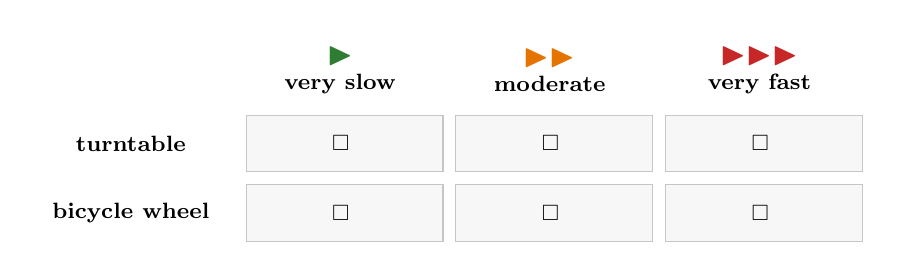
\begin{tikzpicture}[baseline]
\matrix[matrix of nodes, ampersand replacement=\&,
  nodes={draw=gray!45, fill=gray!6, minimum width=2.5cm, minimum height=0.72cm, font=\footnotesize, anchor=center, align=center},
  column sep=1.5mm, row sep=1.5mm,
  row 1/.style={nodes={draw=none, fill=none, font=\footnotesize\bfseries}},
  column 1/.style={nodes={draw=none, fill=none, font=\footnotesize\bfseries}}]{
   \& \shortstack{{\large\textcolor{good}{$\blacktriangleright$}}\\ very slow} \& \shortstack{{\large\textcolor{orange!90!black}{$\blacktriangleright\blacktriangleright$}}\\ moderate} \& \shortstack{{\large\textcolor{bad}{$\blacktriangleright\blacktriangleright\blacktriangleright$}}\\ very fast} \\
  turntable \& $\square$ \& $\square$ \& $\square$ \\
  bicycle wheel \& $\square$ \& $\square$ \& $\square$ \\
};
\end{tikzpicture}
\end{frame}

\begin{frame}{Bottom line}
\begin{block}{Trustworthy}
Same video $\to$ same answer: one locked format, zero broken files, and \gd{0.2--0.4\%} agreement with a real gyroscope.
\end{block}
\begin{block}{The core idea}
The AI \emph{looks}; fixed, vetted code \emph{computes}. Correctness is now \gd{enforced by the system}, not merely requested in a prompt.
\end{block}
\begin{block}{And faster}
$\sim$30 min $\to$ $\sim$8 min per job, with runaway jobs bounded and logs compressed.
\end{block}
\end{frame}

\end{document}
